%   MSc Business Analytics Dissertation
%
%   Title:     Aaa Bbbbbbb Cccccccccc
%   Author(s): Xxxxxx Xxxxxxxxx and Yyy Yyyyyyyyy
%
%   Chapter 6: Discussion
%
%   Change Control:
%   When     Who   Ver  What
%   -------  ----  ---  --------------------------------------------------------------
%   11Feb11  AB    0.1  Begun 
%

\chapter{Discussion}\label{C.Discussion}
\section{Introduction}\label{S.Discussion.intro}
\begin{center}
\begin{figure}[!htb]
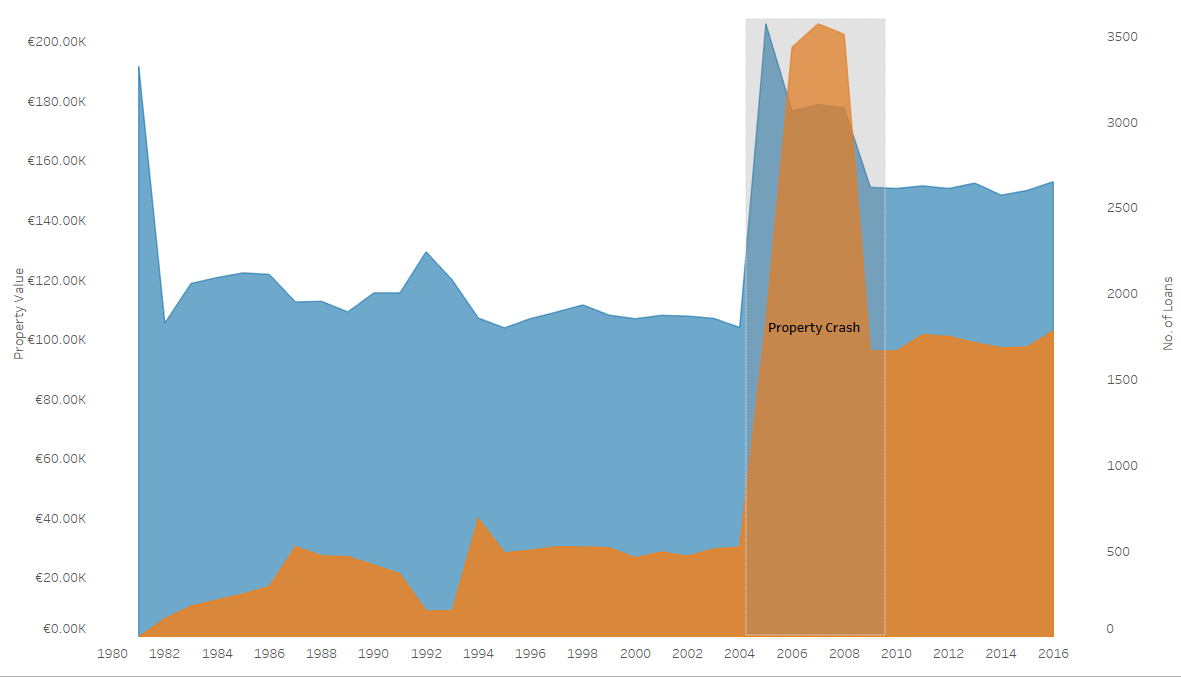
\includegraphics[scale=0.3]{crash1.png}
\centering
\caption{Irish Property Crash}{\textbf{Source:} Tableau Professional v10}
\label{fig:crash1}
\end{figure}
\end{center}
This chapter presents the detailed discussion and analysis of patterns and trends discovered during this research work. Keeping the interest of every stakeholder from bank officer to auditors, an attempt has been build simplicity in the business dashboard so that end user can use it efficiently to drive the business decision. When it was discovered that original data is not appropriate from the predictive modelling perspective, the modified data has been used throughout this research work. All analysis has been presented considering modified data set.

\section{Patterns \&  Analysis}

Since the property crash (2007-2010) average property price and the number of loan applications has been reduced as it can be seen in fig \ref{fig:crash1}. Earlier the average property was \euro 120K then it increased by 100\%.

\begin{center}
\begin{figure}[!htb]
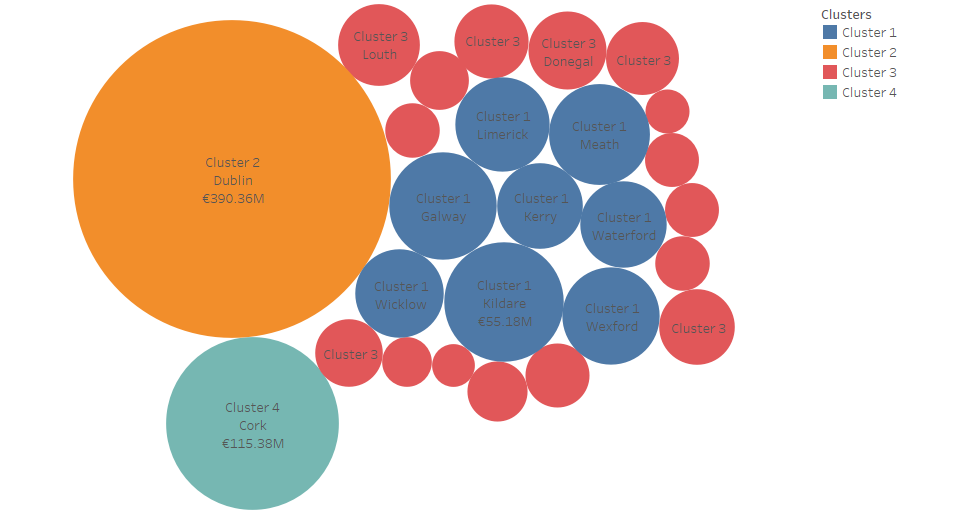
\includegraphics[scale=0.4]{clustero.png}
\centering
\caption{County Cluster}{\textbf{Source:} Tableau Professional v10}
\label{fig:clustero}
\end{figure}
\end{center}

k-Mean algorithm is used to cluster twenty six(26) counties among four cluster based on loan balance, as Ireland property market vary a lot in county. Co. Dublin is classified into cluster \#2 and Co. Cork is classified into cluster \#4 has highest outstanding loan balance. As shown in fig. \ref{fig:cluster} 8 counties are in cluster \#1 and 16 counties with least outstanding loan balance classified into cluster \#3.

\begin{center}
\begin{figure}[!htb]
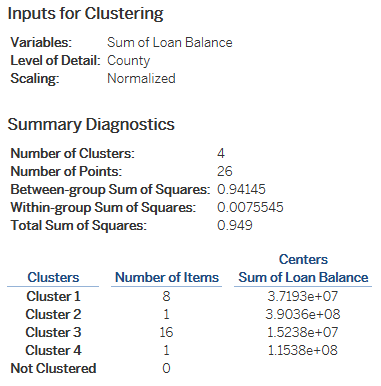
\includegraphics[scale=0.5]{cluster.png}
\centering
\caption{Clustering Results}{\textbf{Source:} Tableau Professional v10}
\label{fig:cluster}
\end{figure}
\end{center}

During data analysis phase, it was noted that the most properties has LTV(Loan-to-value) ratio between 60 - 80\%. There are few properties with LTV higher than 100\%.
In fig. \ref{fig:ltv}
\begin{center}
\begin{figure}[!htb]
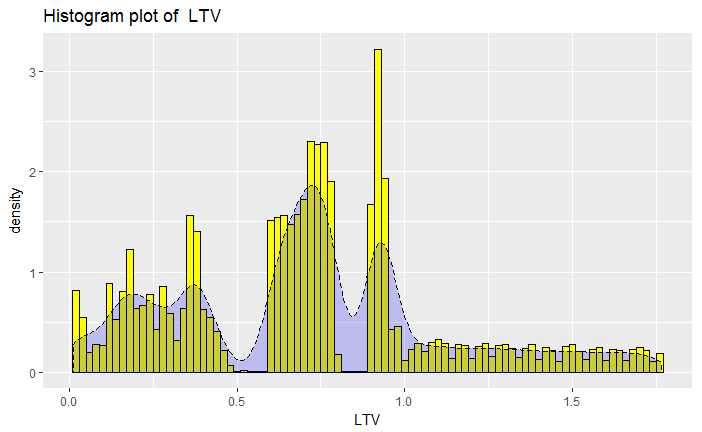
\includegraphics[scale=0.5]{ltv.png}
\centering
\caption{Loan to Value histogram}{\textbf{Source:} R Studio ggplot()}
\label{fig:ltv}
\end{figure}
\end{center}

\begin{center}
\begin{figure}[!htb]
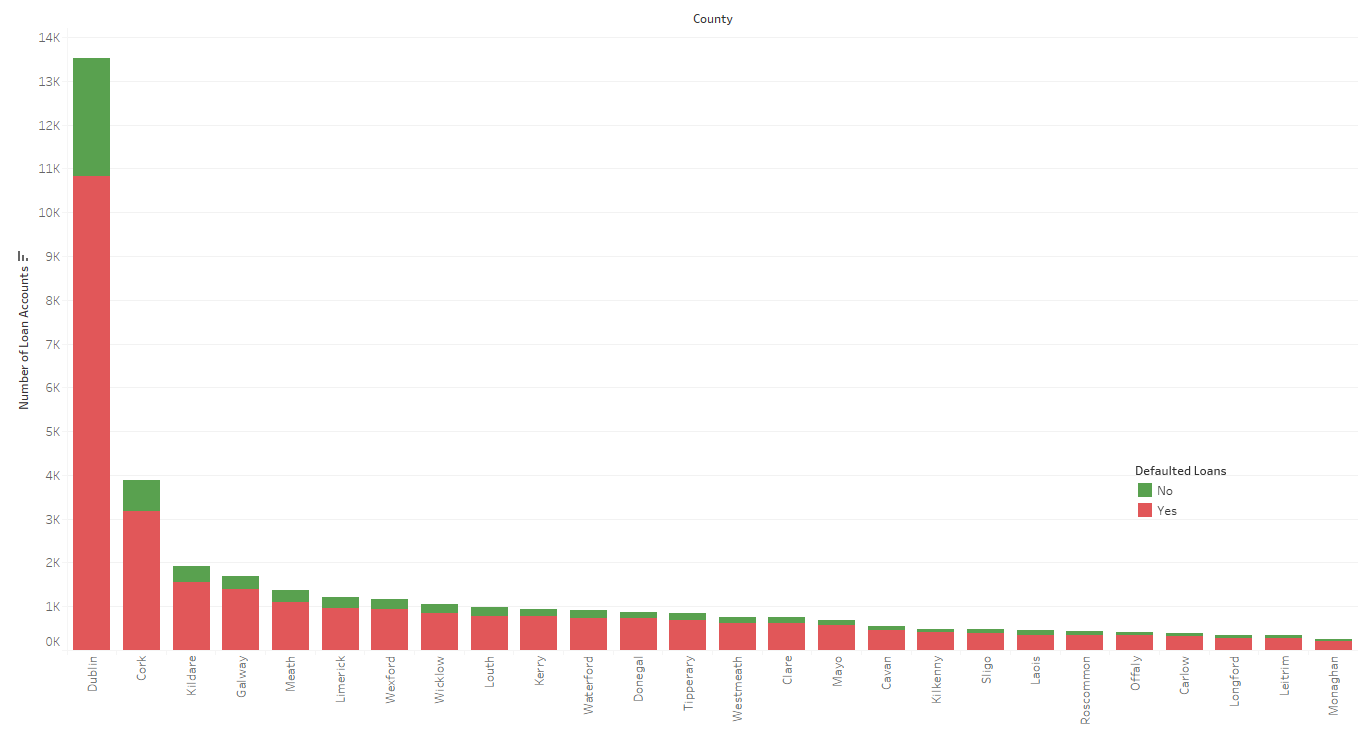
\includegraphics[scale=.4]{countynumber.png}
\centering
\caption{Number of account county wise}{\textbf{Source:} Tableau Pro}
\label{fig:tableaucounty}
\end{figure}
\end{center}

A total number of accounts in the normalized data set was 273,000 , and most numbers of default and loan account were from County Dublin and Cork as seen in fig. \ref{fig:tableaucounty}.

\section{Statistical Analysis}

Descriptive analysis has been performed using SPSS tool to get better understanding of data and take required steps for data preprocessing.

\begin{center}
\begin{figure}[!htb]
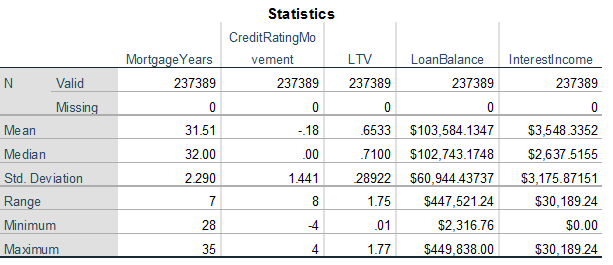
\includegraphics[scale=0.7]{stats1.png}
\centering
\caption{Analysis of Significant variables - 1}{\textbf{Source:} SPSS}
\label{fig:stats1}
\end{figure}
\end{center}


\begin{center}
\begin{figure}[!htb]
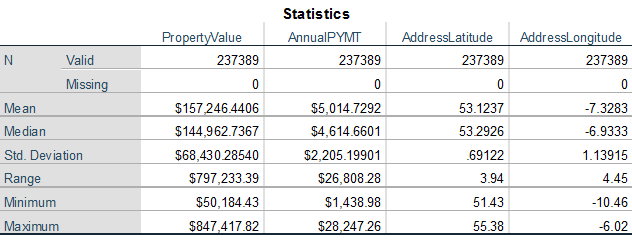
\includegraphics[scale=0.7]{stats2.png}
\centering
\caption{Analysis of Significant variables - 2}{\textbf{Source:} SPSS}
\label{fig:stats2}
\end{figure}
\end{center}



\section{Dashboard}
Considering the day-to-day requirement of stakeholders at KPMG, three business dashboards are designed using Tableau software. Main response to build dashboard using Tableau,as it allow the easy integrations with predictive model from R engine and provides a better means to visualize prediction and forecast.

\begin{center}
\begin{figure}[!htb]
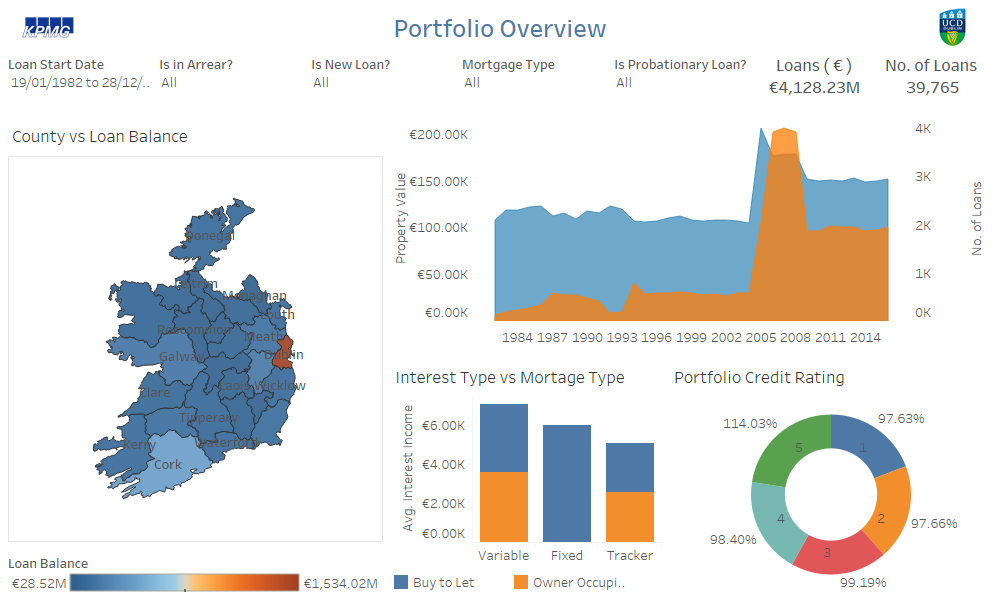
\includegraphics[width=\textwidth]{Overview.png}
\centering
\caption{Portfolio Overview}{\textbf{Source:} Tableau Professional v10}
\label{fig:overview}
\end{figure}
\end{center}


\textbf{Portfolio Overview}\\
Portfolio overview dashboard is built to allow auditors and credit analysts to analyse overall existing loan portfolio registered under a bank. This dashboard allows the user to perform a detailed analysis by selecting various combinations of variables from filters such as:
\begin{itemize}
\item Loan Start Date: User can view selective number of loan account based on the start date of a account
\item Is in Arrears?: Does a loan account has any outstanding repayment in last one year?
\item Mortgage Type: For what purpose mortgage has been buy-to-let or owner occupied?
\item Is probationary Loan?: Has the loan account been converted to probationary loan
\end{itemize}

The geospatial map allows analyst to view loan balance for each county, along with a time-series analysis of property price and number of accounts for past three decades. Using interest type vs mortgage type user can identify which type of interest is giving more income to banks.

\begin{center}
\begin{figure}[!htb]
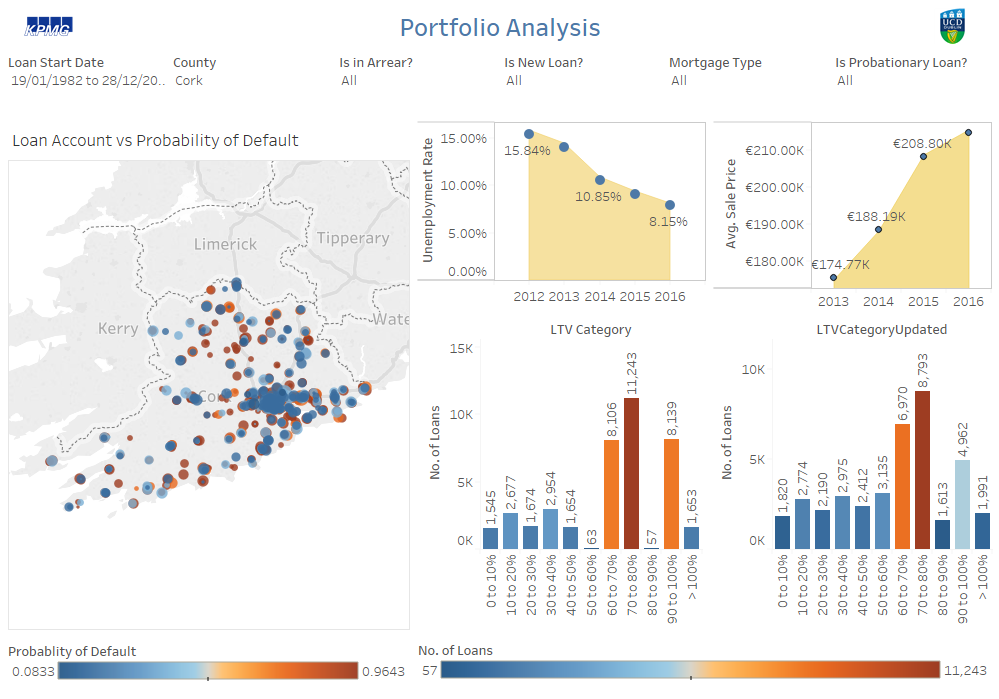
\includegraphics[width=\textwidth]{Analysis.png}
\centering
\caption{Portfolio Analysis}{\textbf{Source:} Tableau Professional v10}
\label{fig:overview}
\end{figure}
\end{center}
\textbf{Portfolio Analysis}\\
Portfolio analysis dashboard allow user to view loan account movement from one LTV (loan to value) category to other, along with unemployment rate and average property sale price in a town. User can select range of property from map using a distance(radius in kms as in fig \ref{fig:dist}) to compare trends in selected neighbourhood.

\begin{center}
\begin{figure}[!htb]
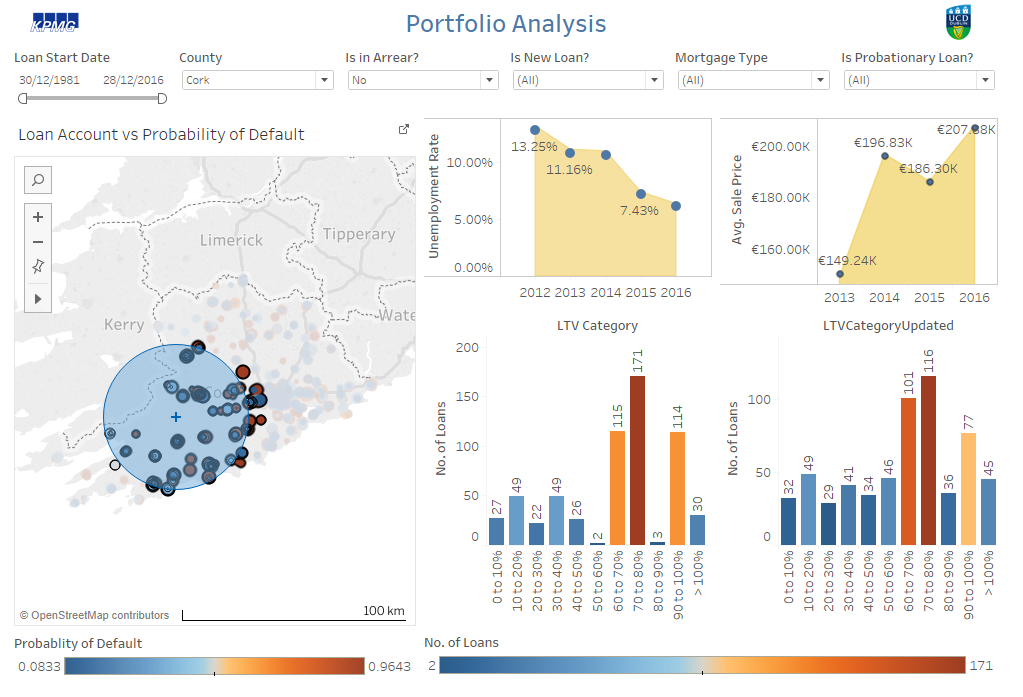
\includegraphics[width=\textwidth]{dist.png}
\centering
\caption{Property Selection using distance}{\textbf{Source:} Tableau Professional v10}
\label{fig:dist}
\end{figure}
\end{center}

By using open source library of R Shiny, a dynamic dashboard has been build which allow user to view property based on clustring. Also user can view street level statstical metrics.

\begin{center}
\begin{figure}[!htb]
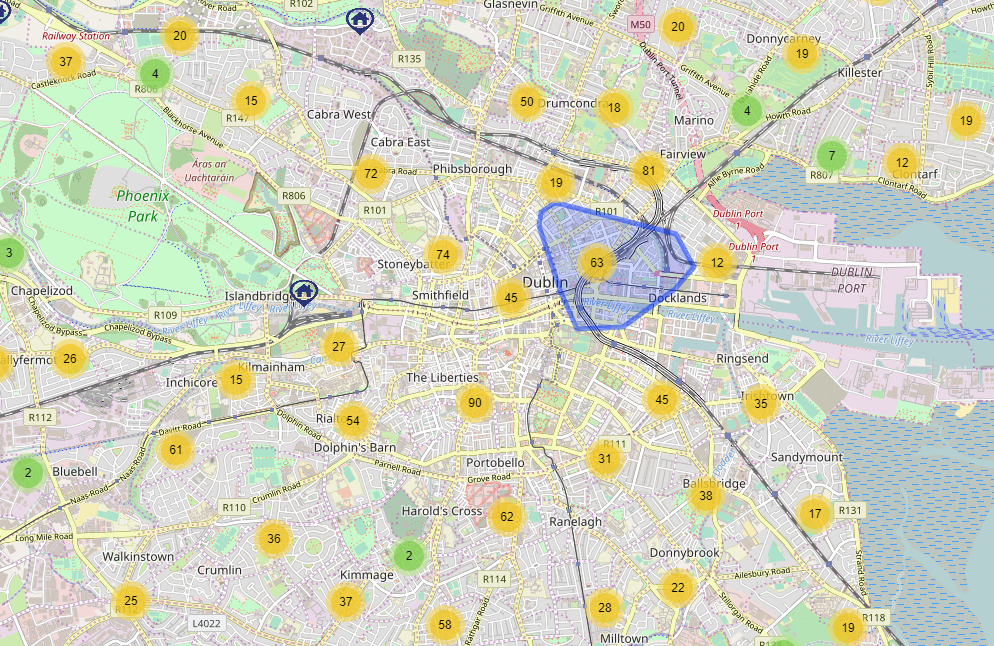
\includegraphics[width=\textwidth]{rmap.png}
\centering
\caption{Dashboard Build using R Shinny}{\textbf{Source:} R Studio}
\label{fig:rmap}
\end{figure}
\end{center}



\section{Success}\label{S.succes}
To measure the performance of this work, a working business dashboard has been given to stakeholder to use it and provide their feedback. Based on their feedback and suggestions dashboard features has been implemented accordingly. The user was given two dashboard design and asked to recommend best one with possible changes and suggestions to further improve usability.

\begin{itemize}
\item \textbf{47\%}Auditors feel this dashboard is extremely useful
\item \textbf{70\%}Feel that geospatial techniques have enhanced credit assessment
\item \textbf{60\%}Likely to recommend this dashboard to colleagues
\end{itemize}